\paragraph{La classe MainActivityViewModel}

\begin{minipage}
    {\linewidth}
    \centering
    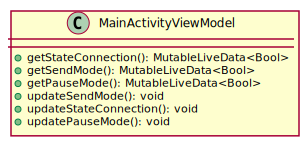
\includegraphics[width=0.80\linewidth]{../schemas/Conception_detaillee/classe_mainActivityViewModel.pdf}
    \captionof{figure}{Diagramme de classe de MainActivityViewModel}
\end{minipage}

\subparagraph{Philosophie de conception \newline} 

\medspace

La classe MainActivityViewModel a pour rôle de de mettre à jour l'affichage des boutons en fonctions des différents états de l'application. 

\subparagraph{Description structurelle \newline}

\medspace

\textbf{Attributs :}

N.A. 

\textbf{Services offerts :}

\begin{itemize}
    \item \textbf{getStateConnection(): MutableLiveData<Bool>} --- Opération qui retourne l'état de la connexion. 
    \item \textbf{getSendMode(): MutableLiveData<Bool>} --- Opération qui retourne l'état du mode d'envoi.
    \item \textbf{getPauseMode(): MutableLiveData<Bool>} --- Opération qui retourne l'état du mode pause ou play du sniffer.
    \item \textbf{updateSendMode(): void } --- Opération qui défini la valeur du mode d'envoi. 
    \item \textbf{updateStateConnection(): void} --- Opération qui défini la valeur de la connexion. 
    \item \textbf{updatePauseMode(): void} --- Opération qui défini la valeur du mode pause ou play du sniffer.
\end{itemize}